% Register Appendix A without creating a mostly empty title page. The embedded
% PDF itself names the role, carries the capture date and contains a clickable
% original-listing link in its footer.
\refstepcounter{section}
\phantomsection
\addcontentsline{toc}{section}{\protect\numberline{\thesection}Job Listing}
\label{sec:Job Listing}
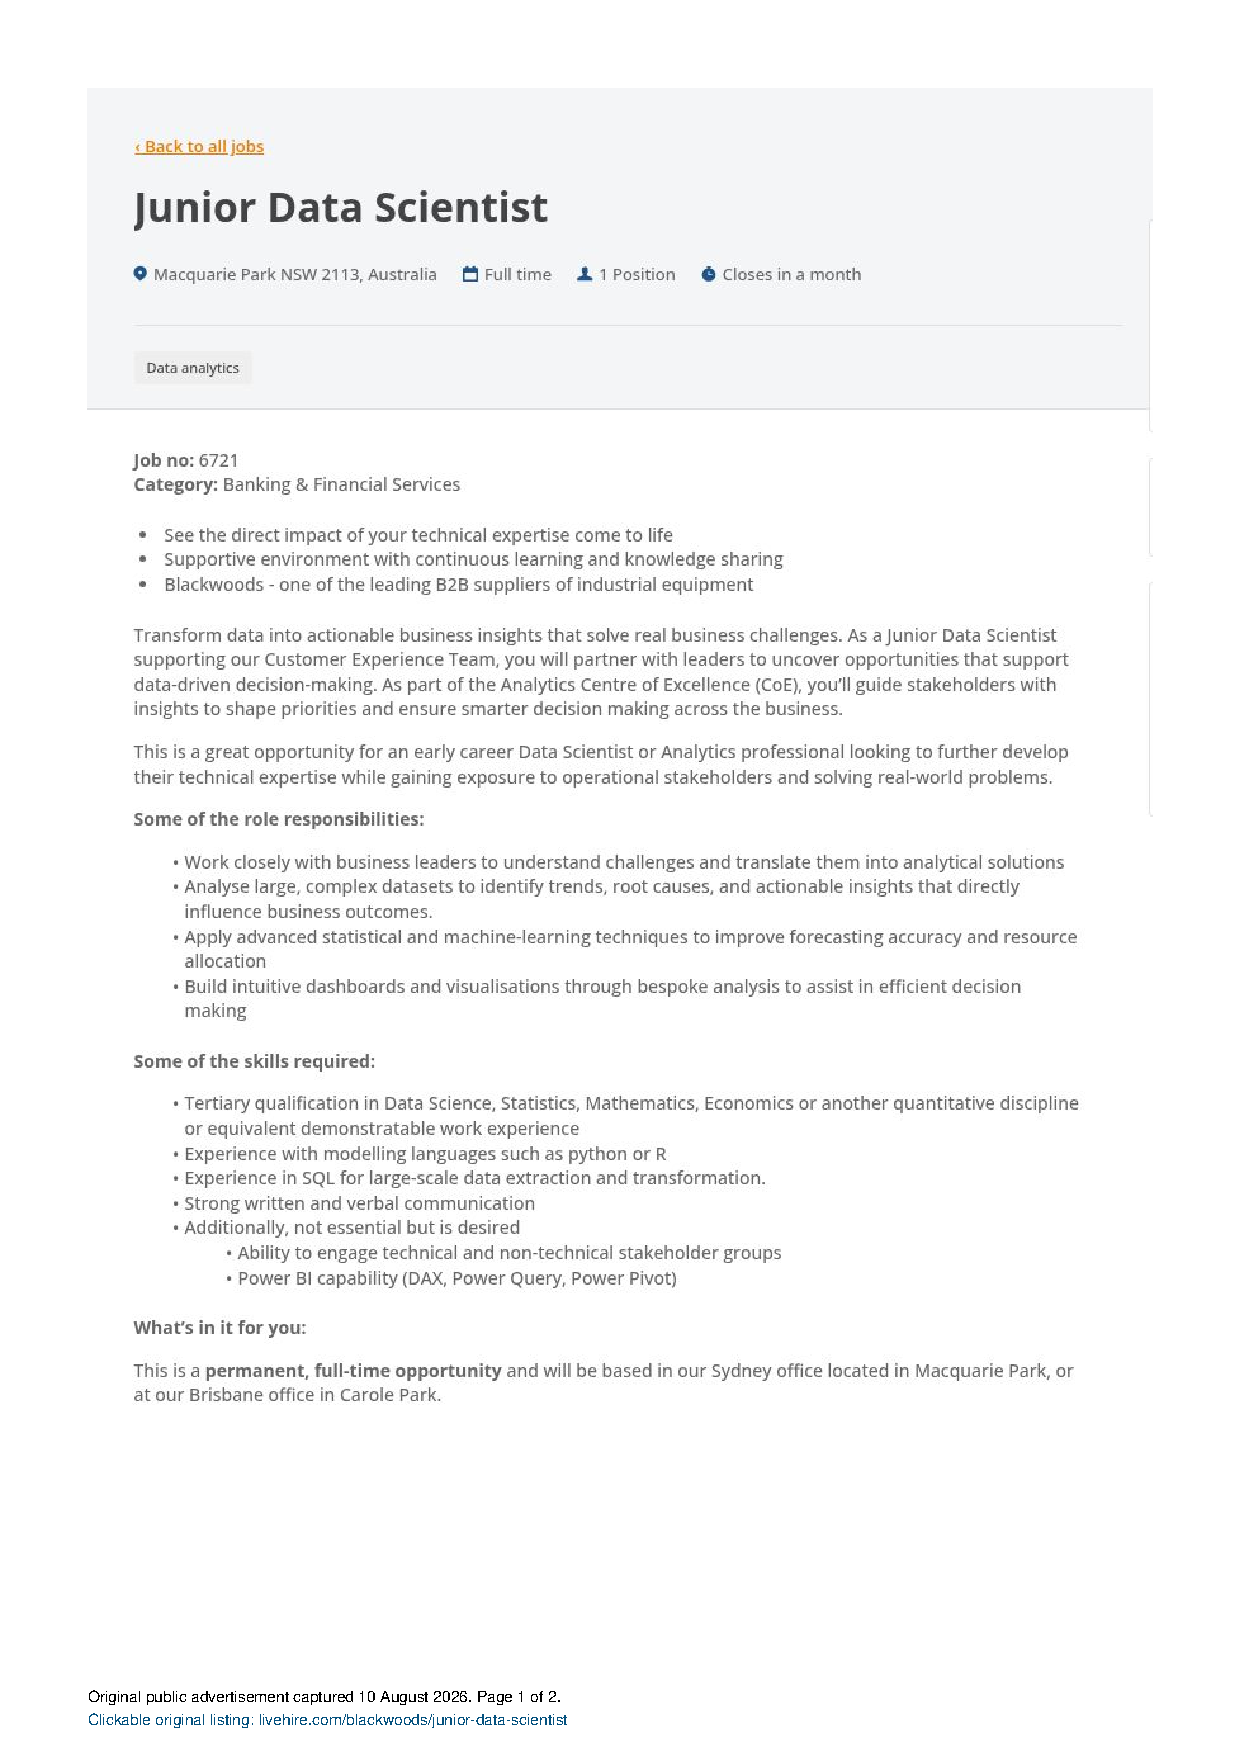
\includepdf[
  pages=-,
  fitpaper=false,
  pagecommand={\thispagestyle{plain}}
]{job_ad_blackwoods.pdf}


%----------------------------------
\section{Link to GitHub Repository}
\label{sec:GitHub}
%----------------------------------

\noindent\textbf{Clickable reproducibility repository:}
\url{\githubprojecturl}

Repository includes the full Python code, dependencies, data source information, processed data, output of models, and all figures used in this report. Raw public data is downloadable from UCI automatically; there is no private or Blackwoods customer data used.


% The cover letter is deliberately the final, unnumbered-looking page so it can
% be extracted and sent as a professional stand-alone letter while retaining an
% appendix label for cross-referencing from the report.
\clearpage
\refstepcounter{section}
\phantomsection
\addcontentsline{toc}{section}{\protect\numberline{\thesection}Cover Letter}
\label{sec:Cover Letter}
\thispagestyle{empty}

\begin{flushright}
\textbf{Yaswanth Gunti}\\
Melbourne, Victoria\\
\href{mailto:s4188617@student.rmit.edu.au}{s4188617@student.rmit.edu.au}\\[0.8em]
10 August 2026
\end{flushright}

\noindent Hiring Manager\\
Blackwoods\\
Macquarie Park, NSW

\medskip
\noindent Dear Hiring Manager,

\medskip
\noindent I am interested in the role of Junior Data Scientist (Vacancy No.~6721), which is available in the Customer Experience Team of Blackwoods. At present, I am enrolled in a Master of Data Science at RMIT University, which makes this role interesting for me.

\medskip
\noindent The RMIT projects illustrate the whole range of competencies that come with the job. The course on Practical Data Science includes preparing a dataset of 4,424 student outcomes, performing the analysis of classification models via cross validation and class sensitive measures and finally formulating actionable conclusions. The course of Advanced Programming saw me developing a reproducible Python process for extracting and integrating XML reviews data with handling of missing, inconsistent and duplicates. My Data Visualisation project using ABS General Social Survey data improved my R and Plotly skills and developed my storytelling capability.

\medskip
\noindent In this particular case study, I expanded upon this experience by analyzing 541,909 retail transaction records and 12,330 Internet sessions. In addition to feature engineering for customers and journeys, I compared regularized logistic regression with a nonlinear support vector machine, quantified uncertainties, and mapped predictions to targeting lifts. This project helped me hone my Python programming skills and data analytics abilities. Most importantly, however, it re-emphasized a critical lesson - a more complicated model should only be considered when providing decision value reliably.

\medskip
\noindent The values of Blackwoods with regard to collaboration, learning, inclusion, and direct impact of business align well with my working style. The Data Science Professional project that involved responsible application of a language model for finance taught me the importance of limitations, evidence, and communication. I would apply this approach in working with business leaders, while developing my skills in SQL and Power BI in the Analytics Centre of Excellence.

\medskip
\noindent It is with great interest that I would like to discuss the contribution that my analysis base, curiosity, and stakeholder-based communication would make toward decision making at Blackwoods.

\medskip
\noindent Yours sincerely,

\medskip
\noindent Yaswanth Gunti
